\chapter{刚体的转动}
\vspace*{-2em}
\thispagestyle{empty}
\section{刚体的转动}
\vspace*{-1em}
\dy[刚体]{GT} 刚体是一种理想模型,受力时不改变形状和体积的物体.\jg
\margin{\\[3em]\kg$\omega_0\,\,$初角速度,\\\kg$\theta\,\,$角位移\\\kg$\alpha\,\,$角加速度}
\par \dy[刚体的转动]{GTDZD}
\begin{equation}
\omega = \omega_0+\alpha t,\quad 
\theta =\omega_0 + \frac{1}{2}\alpha t,\quad 
\omega^2-\omega_0^2=2\alpha\theta,\quad 
\end{equation}

\section{转动定律}
\vspace*{-1em}
\dy[刚体的角动量]{GTDJDL}
\begin{equation}
L=J\omega
\end{equation}
\par \dy[转动定律]{ZDDL}质点系的角动量沿固定轴(取$z$轴)的分量式,
\margin{\\[-1em]$M_z$刚体对转轴的力矩之和(代数值)\\$L_z$刚体对转轴的角动量\\$J\,\,$刚体对转轴的转动惯量\\$\omega\,\,$刚体绕转轴转动的角速度}
\begin{equation}
M_z=\frac{\d L_z}{\d t}=J\frac{\d \omega}{\d t}
\end{equation}
去掉下标,可以写成
\begin{equation}
M=J\frac{\d \omega}{\d t}=J\alpha
\end{equation}
\begin{table}[!htb]
	\centering
	\caption{一些均匀转动刚体的转动惯量}
		\renewcommand\arraystretch{2}
	\setlength{\tabcolsep}{6mm}{
		\begin{tabular}{cccc}
			\midrule[1.4pt] 
			& & & \vspace*{-4.6em}\\
			刚体形状 &轴的位置 &图示   &转动惯量\\
			& & & \vspace*{-4em}\\
			\midrule
			& & & \vspace*{-4.3em}\\
			细杆 & $\,\,\,\,$通过一端垂直于杆 &\makecell[c]{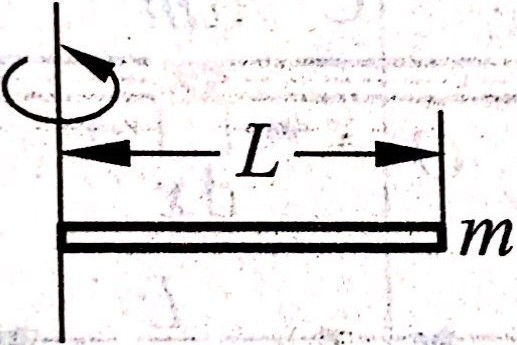
\includegraphics[scale=0.07]{picture/转1.jpg}}   & $\disp\frac{1}{3}mL^2$\\
			\hline
			& & & \vspace*{-4.3em}\\
			\makecell[c]{细杆}  & 通过中点垂直于杆 & \makecell[c]{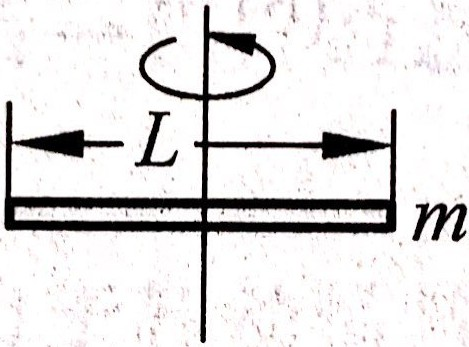
\includegraphics[scale=0.08]{picture/转2.jpg}}  &  $\disp\frac{1}{12}mL^2$\\
			\hline
			\makecell[c]{薄圆环\\(薄圆筒)} & \makecell[c]{通过环心垂直于环面 \\ (中心轴)}& 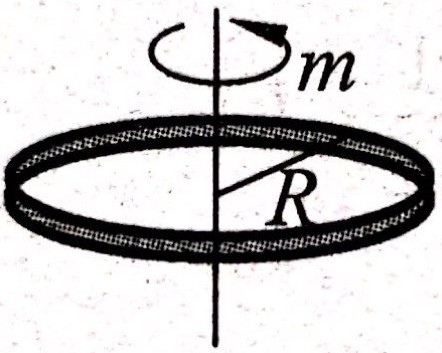
\includegraphics[scale=0.07]{picture/转3.jpg} & $mR^2$\\
			\hline
			\makecell[c]{ $\,\,$圆盘\\$\,\,$(圆柱体)} & \makecell[c]{通过盘心垂直于盘面 \\ (中心轴)} & \makecell[c]{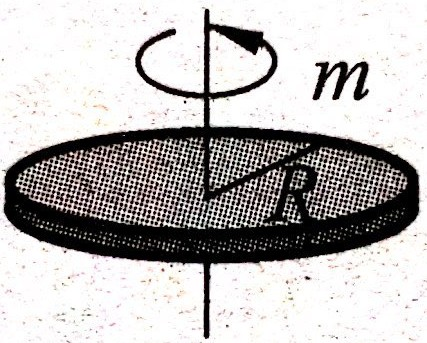
\includegraphics[scale=0.07]{picture/转4.jpg}} &  $\disp\frac{1}{2}mR^2$\\
			\hline
			& & & \vspace*{-4.3em}\\
			$\,\,$薄球壳 & 直径 & \makecell[c]{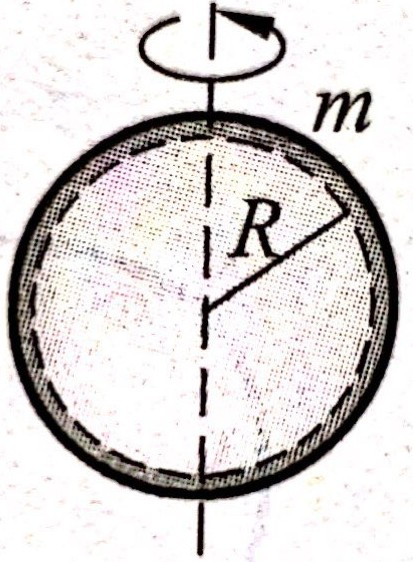
\includegraphics[scale=0.05]{picture/转5.jpg}}&$\disp\frac{2}{3}mR^2$ \\
			\hline
			& & & \vspace*{-4.3em}\\
			球体 &直径 & \makecell[c]{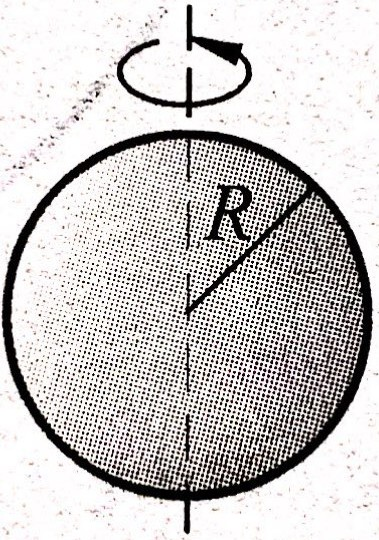
\includegraphics[scale=0.05]{picture/转6.jpg}}&$\disp\frac{2}{5}mR^2$ \\
			\bottomrule[1.4pt]  
		\end{tabular}  
	}
	\renewcommand\arraystretch{1}
	\label{一些均匀转动刚体的转动惯量}
\end{table} 
\newpage

\par \dy[转动惯量]{ZDGL}决定于刚体的质量相对于转轴的分布
\margin{常见的刚体的转动惯量见上页表\ref{一些均匀转动刚体的转动惯量}.}
\margin{$r$为质点$\d m(m_i)$到转轴的垂直距离}
\begin{equation}
J=\sum m_ir_i^2 \quad \mbox{或} \quad J=\int \bm{r}^2\d m
\end{equation}
\par \dy[平行轴定理]{PXZDL}
\margin{\\[-0,5em]\kg$J_C$表示刚体对于通过其质心$C$的轴的转动惯量.}
\begin{equation}
J=J_C+md^2
\end{equation}

\section{角动量守恒}
\dy[角动量守恒定律]{JDLSHDL}
\begin{equation}
M_z=\frac{\d L_z}{\d t} = 0 \quad  \Longleftrightarrow \quad L_z=0.
\end{equation}
\par 对于一个质点系,如果它受的对于某个固定轴的合外力矩为0,则它对于这一固定轴的角动量保持不变。

\section{刚体转动的功和能}
\dy[力矩的功]{LJDG}
\begin{equation}
A=\int_{\theta_1}^{\theta_2}M\d \theta 
\end{equation}

\dy[转动动能]{ZDDN}
\begin{equation}
E_k=\frac{1}{2}J\omega^2
\end{equation}

\dy[刚体的重力势能]{GTDZLSN}
\begin{equation}
E_p=mgh_C
\end{equation}
\par 一个不太大的刚体的重力势能和它的全部质量集中在质心时所具有的势能一样。\jg\jg 

\dy[动能定理]{DNDL}
\begin{equation}
A_{AB}=\frac{1}{2}J\omega_B^2+\frac{1}{2}J\omega_A^2
\end{equation}


\dy[机械能守恒定律]{JXNSHDL}对封闭的保守系统(只有保守力做功),
\begin{equation}
E_k+E_p=C\,\mbox{常量}
\end{equation}

